\chapter{収差と回折限界}
\label{chap:basic_matters}
分光器の分解能は収差と回折限界の影響を受ける.
% 本章では分光器の分解能を考えるうえで大切な要素である収差の評価を行う.
本章では,高度な光線追跡及びスポット解析が行えるソフトウェアであるOSLOを用いて収差と回折限界が分解能に与える影響についてシミュレーションを行う.
スポット解析とはレンズや凹面鏡などで集光した際の結像面での光線の集まり方を調べることである.
この際の結像面での光の分布図をスポット図という.
図\ \ref{fig:OSLO_spot_example}に,OSLOによって作成した光線追跡図及びスポット図の例として焦点距離486.2 mm,有効径100 mmの凸レンズに波長587.6 nmの平行光を入射させた際のシミュレーション結果を示す.
\floatsetup[figure]{style=plain,subcapbesideposition=top}
\begin{figure}
    \sidesubfloat[]{
        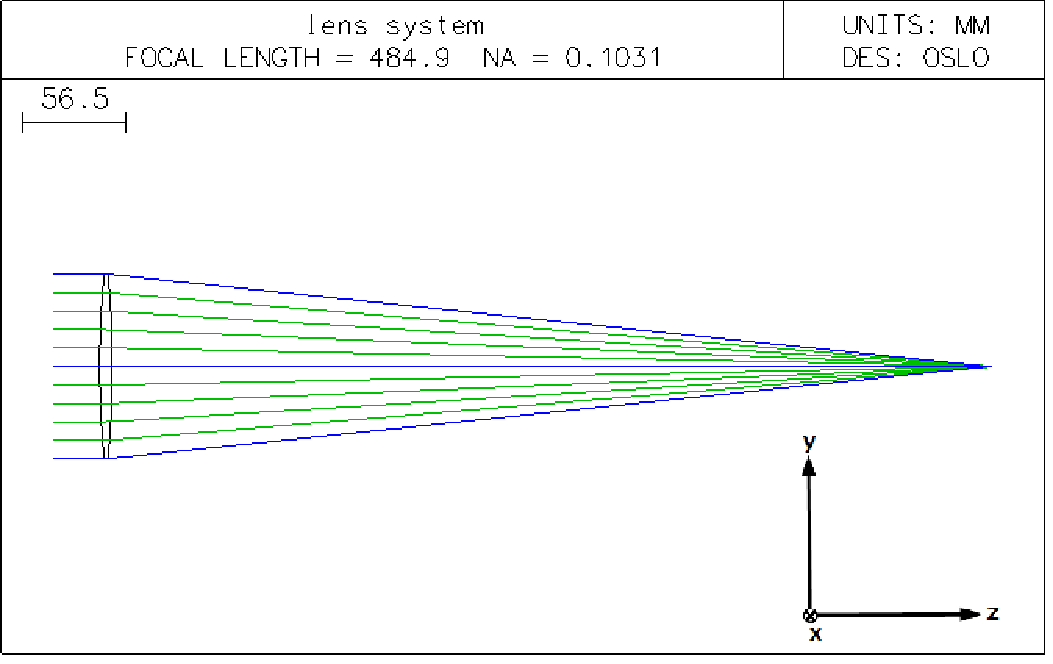
\includegraphics[scale=0.35]{figure/OSLO_raytrace_example.pdf}}
    \sidesubfloat[]{
        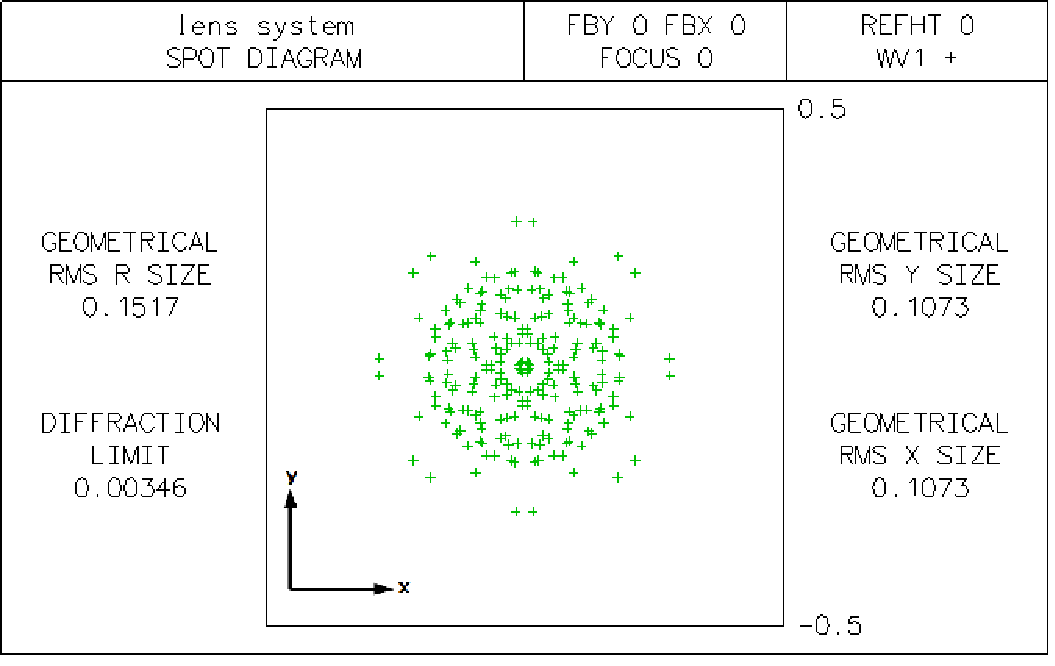
\includegraphics[scale=0.35]{figure/OSLO_spot_example.pdf}}
    \caption{OSLOによるシミュレーションの例(焦点距離486.2 mm,有効径100 mmのレンズを設定) \\
    \centering(a)光線追跡図,
    (b)焦点面でのスポット図}
    \label{fig:OSLO_spot_example}
\end{figure}
ここで,図中にあるように座標系を設定した.
本研究におけるOSLOによるシミュレーションにおいて座標系は図\ \ref{fig:OSLO_spot_example}と同じ設定とし,光は常にz軸負の方向からz軸に平行に入射されるものとする.
図中の数字の単位は全てmmであり,これ以降に出てくる光線追跡図及びスポット図についても同様であるとする.


% ここで,図\  \ref{fig:OSLO_spot_example}(b)のようにある面に対して光を結像させたとき光の分布は二次元のガウス関数で近似できるとすると,スポット図にあるGEOMETRICAL RMS R SIZE($rms_r$と置く)は半径方向の二乗平均平方根であり,ガウス関数の標準偏差$\sigma$に対応する.
% この結像の大きさ$\phi$を光の分布図をガウス関数に近似した際の半値全幅と定義する.
% ガウス関数において半値全幅($FWHM$)は
% \begin{eqnarray}
%      FWHM &=& 2\sigma\sqrt{2\log2} \\
%      &\simeq&2.35\sigma
% \end{eqnarray}
% とできるため,結像の大きさ$\phi$は$2.35rms_r$となる.
% OSLOによるシミュレーションで求められた結像の大きさ$\phi$のことを以下ではスポットサイズと呼ぶこととする.


\section{収差}
レンズや凹面鏡を用いて平行光を集光させる際,一点に結像させるのが理想であるが現実には不可能であり像には歪みやぼけが生じる.
その歪みやぼけのことを収差という.
収差は大きく分けて波長に依存する色収差と,波長に依存しない単色収差に分類できる.
単色収差のなかで特に影響の大きい5つの収差のことをザイデル収差と呼び,球面収差,コマ収差,非点収差,像面湾曲,歪曲収差がある.
ザイデル収差の中で同軸に光が入射した際でも発生するものは球面収差のみで,他の収差は非同軸系で発生する軸外収差である\cite{syuusa}.

\subsection{色収差}
% 色収差はレンズ特有のものである.
% レンズの媒質であるガラスなどの屈折率が波長によって変化することから生まれる焦点距離のずれのことである.
色収差とは波長にとって物質の屈折率が異なるために発生する焦点距離のずれのことである.
そのため,光を反射することで集光を行なっている凹面鏡では色収差は存在しない.
対して,レンズには色収差があり白色光を入射すると,波長の短い青色光の焦点が波長の長い赤色光の焦点よりも短くなる.
そのためレンズに白色光を入射させたとき結像面において色のにじみが発生する\cite{irosyuusa}.

% https://www.jstage.jst.go.jp/article/jpnjvissci/29/1/29_29.3/_pdf/-char/en


\subsection{球面収差}
球面収差とはレンズや凹面鏡の面が球面であることによって生じる収差のことである.
ここではレンズに平行光を入射させたときを例に球面収差の説明を行う.
図\ \ref{fig:kyuumensyuusa_example}に焦点距離が29.7 mm,有効径が20 mmのレンズに波長587.6 nmの平行光を入射させるときの光線追跡図を示す.
\begin{figure}[htbp]
    \centering
    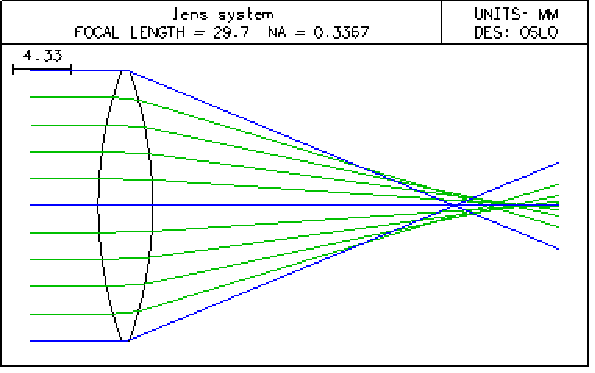
\includegraphics[scale=0.8]{figure/kyuumensyuusa_example.pdf}
    \caption{球面収差が発生している様子}
    \label{fig:kyuumensyuusa_example}
\end{figure}
レンズに入射する各光線で光軸からの距離が大きい光線ほどレンズ面に対する入射角が大きくなり光の屈折が大きくなる.
その結果,入射光線が光軸から離れるほどレンズ近くで焦点を持つ.
これによりレンズの光軸近くに入射する光と光軸から離れた所に入射する光で焦点の位置に差が生じる.



\subsection{コマ収差}
% コマ収差とは彗星のように尾を引いてぼやける収差のことである.
コマ収差はレンズや凹面鏡に対して斜めに光が入射することによって生じる収差である.
コマ収差が発生している様子の例として図\ \ref{fig:koma_syuusa}に焦点距離が100 mm,有効径が30 mmの凹面鏡で波長587.6 nmの平行光を軸外反射によって光軸を30°曲げて集光している様子を示す.
\floatsetup[figure]{style=plain,subcapbesideposition=top}
\begin{figure}
    \sidesubfloat[]{
        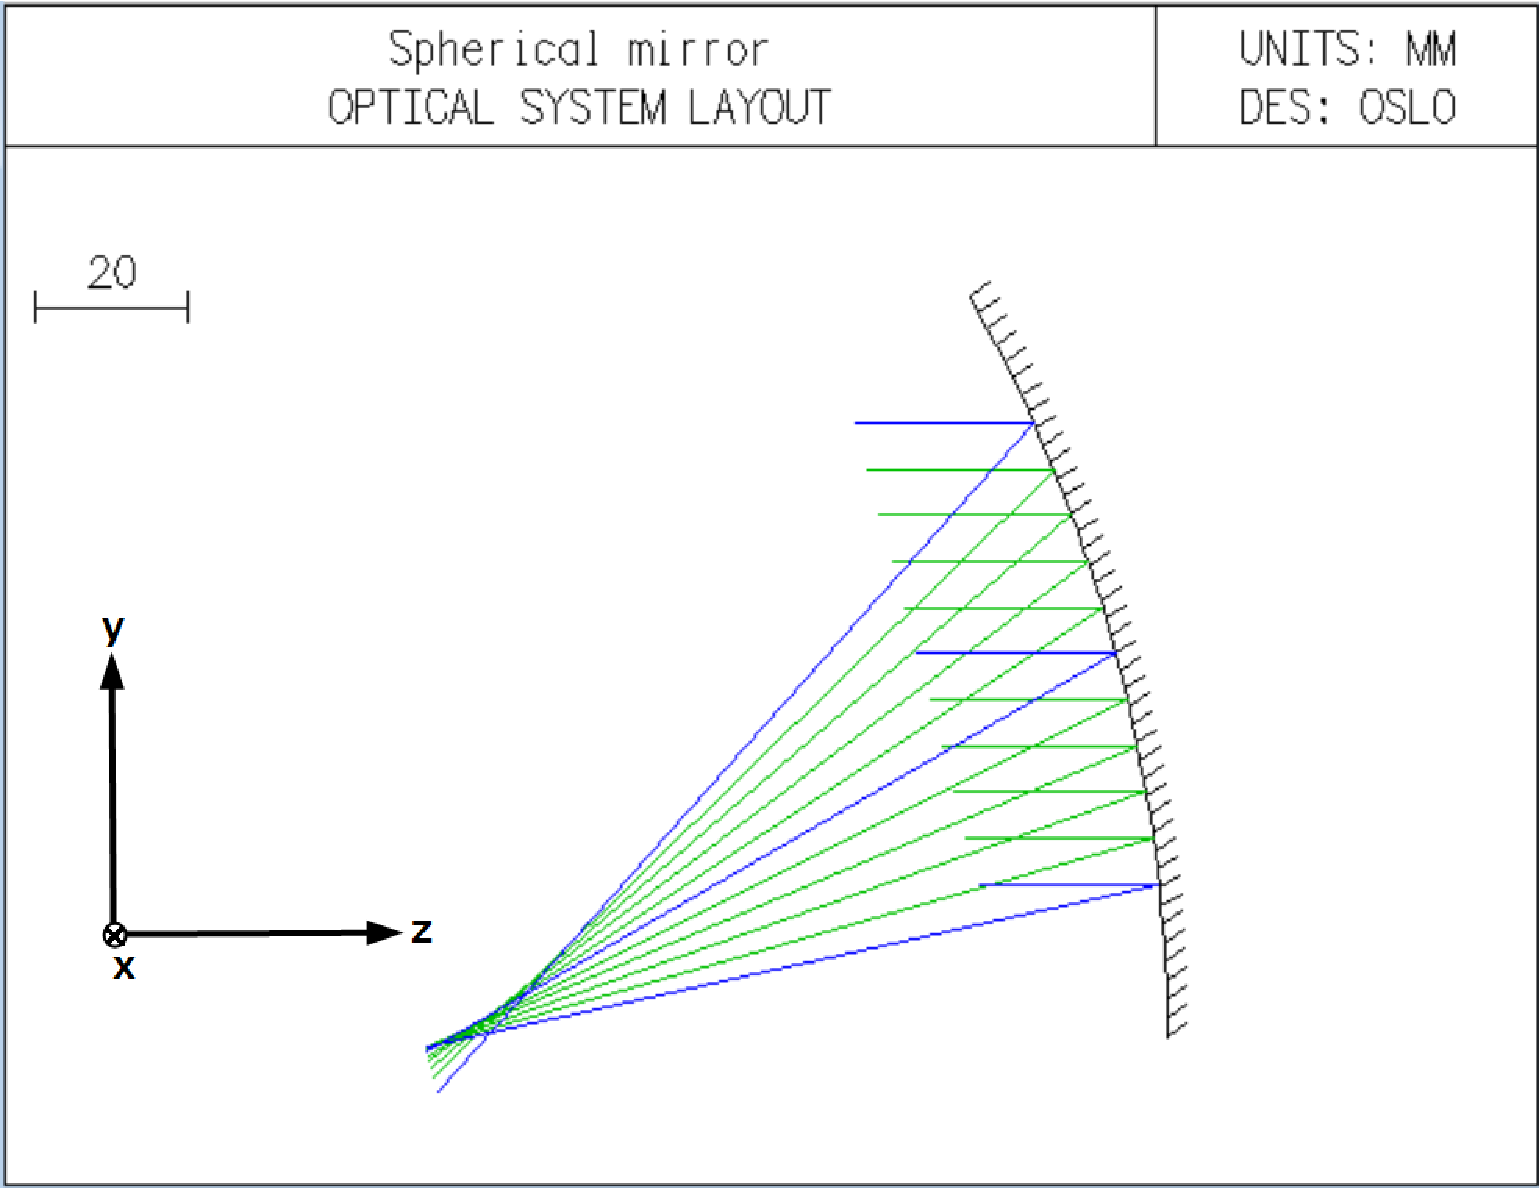
\includegraphics[scale=0.2]{figure/koma_syuusa_zahyou.pdf}}
    \sidesubfloat[]{
        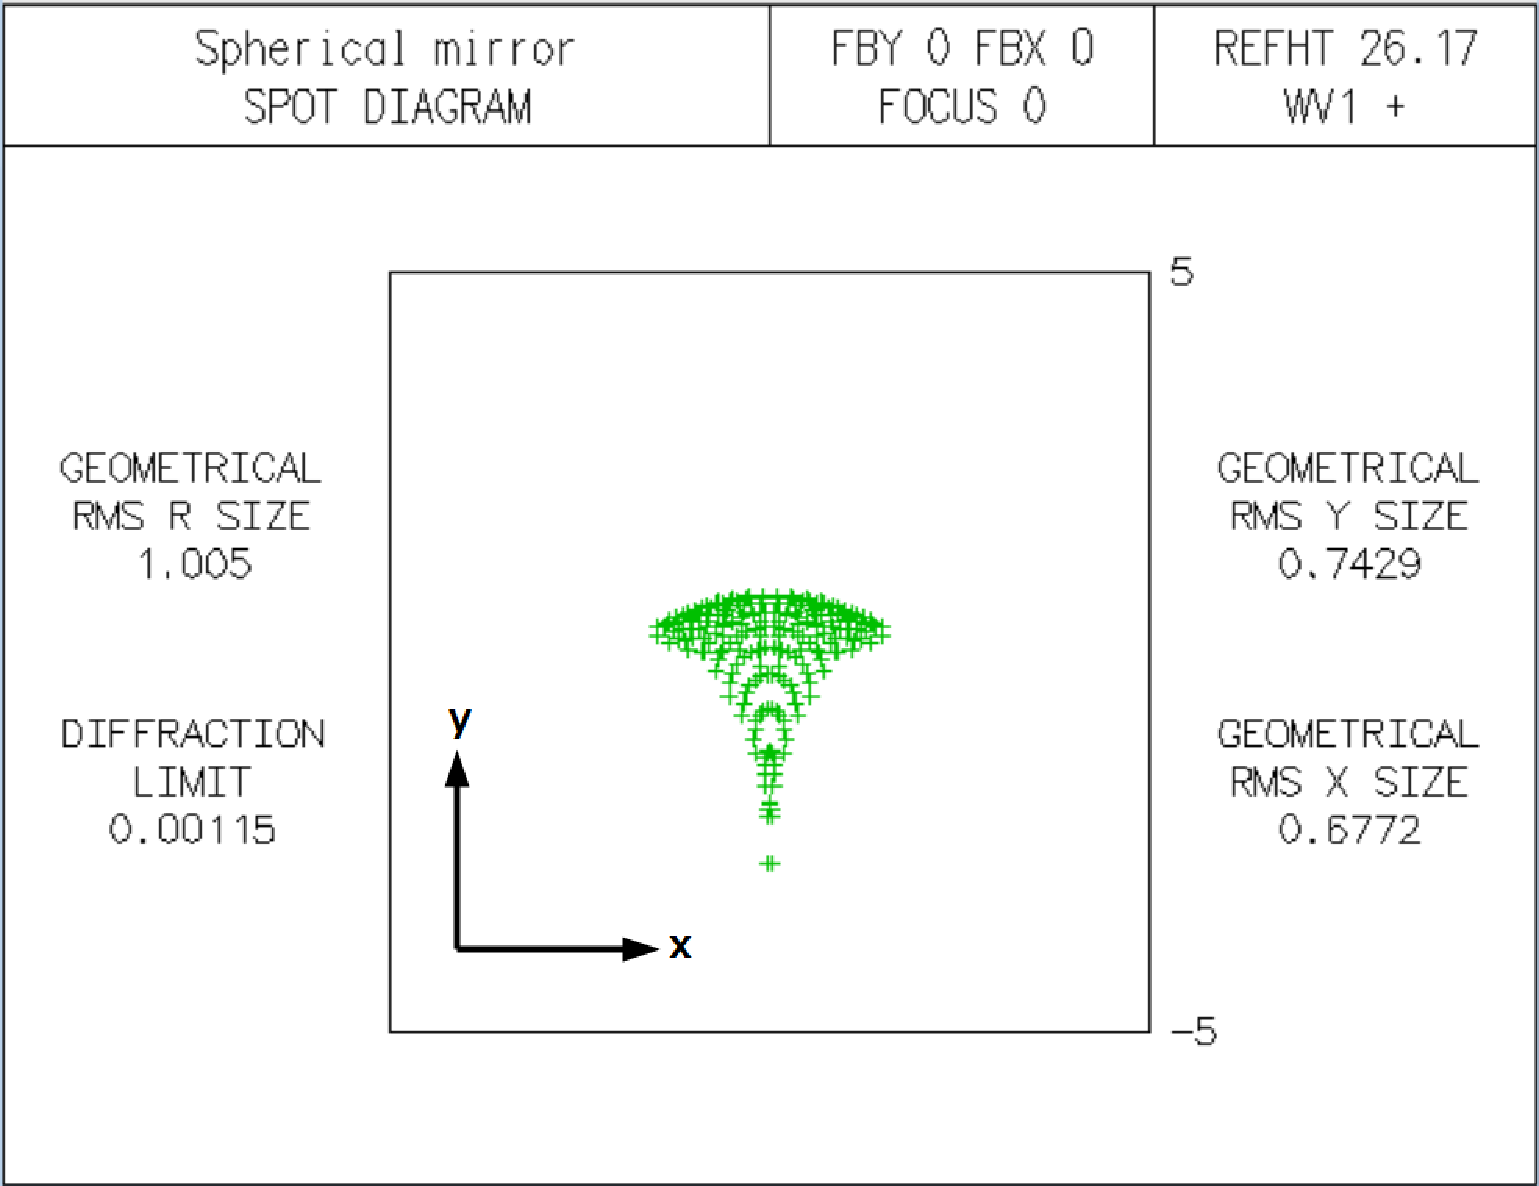
\includegraphics[scale=0.2]{figure/koma_syuusa_spot_zahyou.pdf}}
    \caption{コマ収差が発生している様子 \\
    (a)光線追跡図,
    (b)焦点面でのスポット図}
    \label{fig:koma_syuusa}
\end{figure}
図\ \ref{fig:koma_syuusa}(a)はこのときの光線追跡図を,図\ \ref{fig:koma_syuusa}(b)は焦点面でのスポット図を表す.
% 図\ \ref{fig:koma_syuusa}(a)を見ると主光線(中心を通る光線)に対して光線が非対称になり,結像面において非対称な像を作る.
% これがコマ収差である.
% 図\ \ref{fig:koma_syuusa}(b)はこの凹面鏡において焦点面のスポット図である.
図\ \ref{fig:koma_syuusa}(b)より像がy軸方向に対して非対称になっていることが分かる.
% これがコマ収差である.
図のような彗星のように尾を引いてぼやけることがコマ収差の特徴である.

\subsection{非点収差}
非点収差とは焦点の合う位置の前後で結像の形(縦横比)が変わってぼける収差である\cite{syuusa}.
ここで焦点距離が1525 mm,有効径が98 mmの凹面鏡に対して波長587.6 nmの光を軸外反射によって4°曲げて集光した際,焦点面からz軸方向に+1 mmずらした面でのスポット図及び焦点面からz軸方向に-1 mmずらした面でのスポット図を図\ \ref{fig:hitensyuusa}(a)(b)に示す.
\floatsetup[figure]{style=plain,subcapbesideposition=top}
\begin{figure}
    \sidesubfloat[]{
        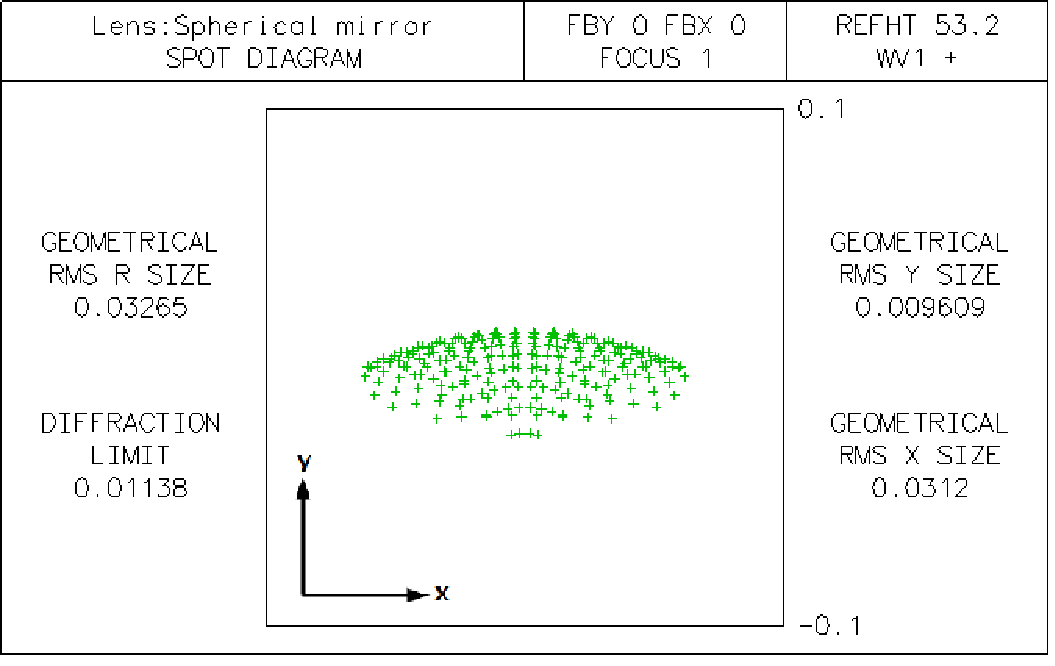
\includegraphics[scale=0.35]{figure/hitensyuusa_1mm.pdf}}
    \sidesubfloat[]{
        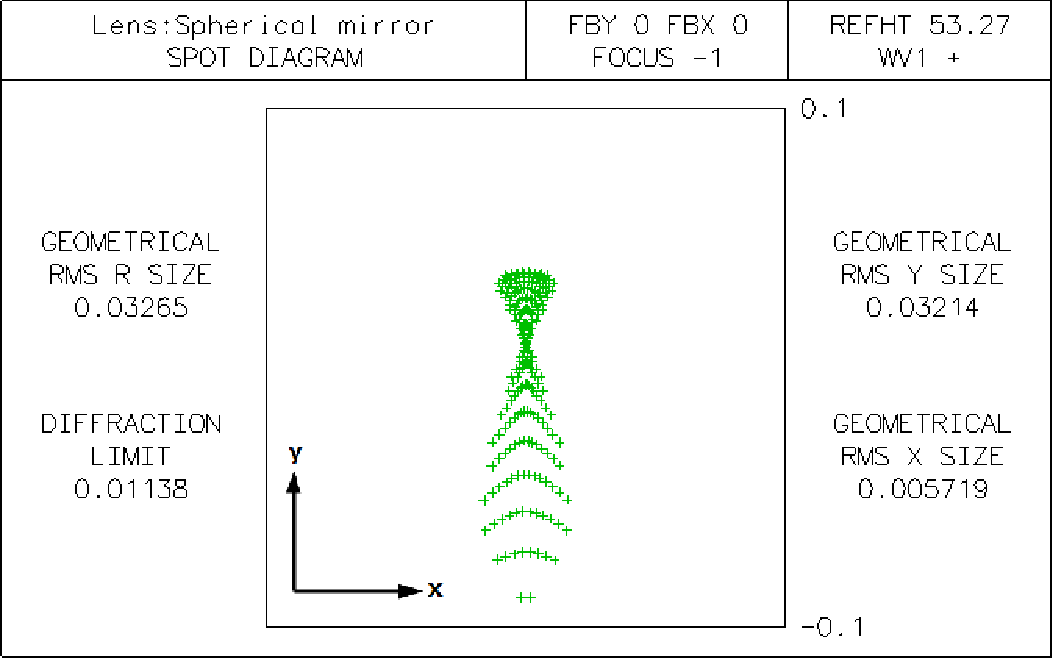
\includegraphics[scale=0.35]{figure/hitensyuusa_-1mm.pdf}}
    \caption[非点収差の様子]{非点収差の様子.焦点距離が1525 mm,有効径が98 mmの凹面鏡で光を軸外反射によって4°曲げて集光した際の焦点面前後のスポット形の変化を表す.\\
    (a)焦点面からz軸方向に+1 mmずらした面でのスポット図,
    (b)焦点面からz軸方向に-1 mmずらした面でのスポット図}
    \label{fig:hitensyuusa}
\end{figure}
図を見るとz軸方向に+1 mmずらした面ではx軸方向に長く結像されているのに対し,z軸方向に-1 mmずらした面ではy軸方向に長く結像されており,焦点前後でぼけ方が変わっていることが分かる.
これは主光線を含むyz平面(子午面)と子午面に垂直なxz平面(球欠平面)内の光線の焦点距離が異なるために発生する.

\subsection{像面湾曲・歪曲収差}
像面湾曲とは,平面から出た光が曲面に結像する収差である.
像面湾曲があると中心で焦点が合っていても周辺で焦点が合わないという現象が起こる.
歪曲収差とは光軸からの距離に応じて像の倍率が異なってくるために起こる歪みのことで,像の形が歪んで見える収差である\cite{nikon}.


% https://www.jstage.jst.go.jp/article/jpnjvissci/36/3/36_40/_pdf/-char/ja

\section{回折限界}
どれだけ収差が抑えられたレンズや凹面鏡を用いても光を一点に集光することはできない.
光の波動性のため回折によって広がってしまうためである.
この回折に制限される分解能の限界のことを回折限界という.

回折限界で結像された光の像は中央部に明るい領域を持ち,その周囲に暗い同心円状輪帯を有するエアリーパターンという回折パターンとなる(図\ \ref{fig:Airy_pattern}).
\begin{figure}[htbp]
    \centering
    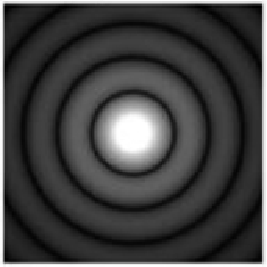
\includegraphics[scale=1.0]{figure/Airy_pattern.pdf}
    \caption{エアリーパターンの模式図\cite{Airy}}
    \label{fig:Airy_pattern}
\end{figure}
中心の明るい領域をエアリーディスクと呼ぶ\cite{airy_disc}.
エアリーディスクの大きさはレンズの焦点における最小の結像サイズである.
エアリーディスクの半径$R$は
\begin{eqnarray}
    R = 1.22\lambda f_{\#}
\end{eqnarray}
と表される.
ここで$\lambda$は光の波長,$f_{\#}$はレンズのf値を表す\cite{airy_disc}.

スペクトルのエアリーディスク部分をガウス関数で近似したときの標準偏差$\sigma$は
\begin{equation}
     \sigma \simeq 0.42\lambda f_{\#}
\end{equation}
と表され\cite{airy_gauss},半値全幅($FWHM$)は
\begin{eqnarray}
     FWHM &=& 2\sigma\sqrt{2\log2} \nonumber \\
     &\simeq&0.99\lambda f_{\#}
\end{eqnarray}
となる.
% https://www.edmundoptics.jp/knowledge-center/application-notes/imaging/limitations-on-resolution-and-contrast-the-airy-disk/




分光器の検出器結像面に回折限界の幅で結像した時が分光器の波長分解の限界である.
その際のスペクトルの波長幅($\delta\lambda$)は逆線分散に先ほどの半値全幅を掛けたものとなる.
ここで,$f_{\#}$はレンズの有効径を$W$とした時$f_{\#}=f/W$であることから
\begin{eqnarray}
     \delta\lambda &=& \frac{\mathrm{cos}{\beta}}{Nmf}\cdot\frac{0.99\lambda f}{W} \nonumber \\
     &=&\frac{0.99 \lambda \mathrm{cos}{\beta} }{mNW}
\end{eqnarray}
とできる.
これが,理論的なスペクトルの最小波長幅である.
% このときの分解能$	d\lambda$を理論分解能といい次式で表される.
% \begin{equation}
    %  d\lambda= \frac{\lambda}{mNW}
% \end{equation}
% ここで$W$は回折格子の有効幅であり,$NW$は回折格子に光が当たっている部分の総刻線数を表す.
% https://www.shimadzu.co.jp/products/opt/guide/05.html




\section{凹面鏡とレンズの結像性能の比較}
本節ではツェルニ・ターナ型分光器のように凹面鏡の軸外反射によって集光・結像する場合と,本実験で採用するアクロマティックレンズを用いて同軸に集光する場合のそれぞれの結像の大きさをOSLOでシミュレーションを行う.
本研究で使用するレンズは焦点距離1525 mm,有効径98 mmのものである.
シミュレーションにおいてレンズと条件を合わせるため,焦点距離を1525 mm,有効径を98 mmの凹面鏡を用いることにした.
また,入射する光は波長587.6 nmの単色光とした.


\subsection{凹面鏡を用いた結像}
ツェルニ・ターナ型分光器で用いられている凹面鏡での集光のシミュレーションを行う.
% 軸外反射での集光はより光軸が大きな角度で曲げられているほど収差は大きくなる.
凹面鏡に平行光を入射し同軸で集光した際の焦点面でのスポット図,軸外反射の角度を2°に設定した際の焦点面でのスポット図,軸外反射の角度を3°に設定した際の焦点面でのスポット図,軸外反射の角度を4°に設定した際の焦点面でのスポット図をそれぞれ図\ \ref{fig:off_axis_spot_0},図\ \ref{fig:off_axis_spot_1},図\ \ref{fig:off_axis_spot_1.5},図\ \ref{fig:off_axis_spot_2}に示す.
\begin{figure}[htbp]
    \centering
    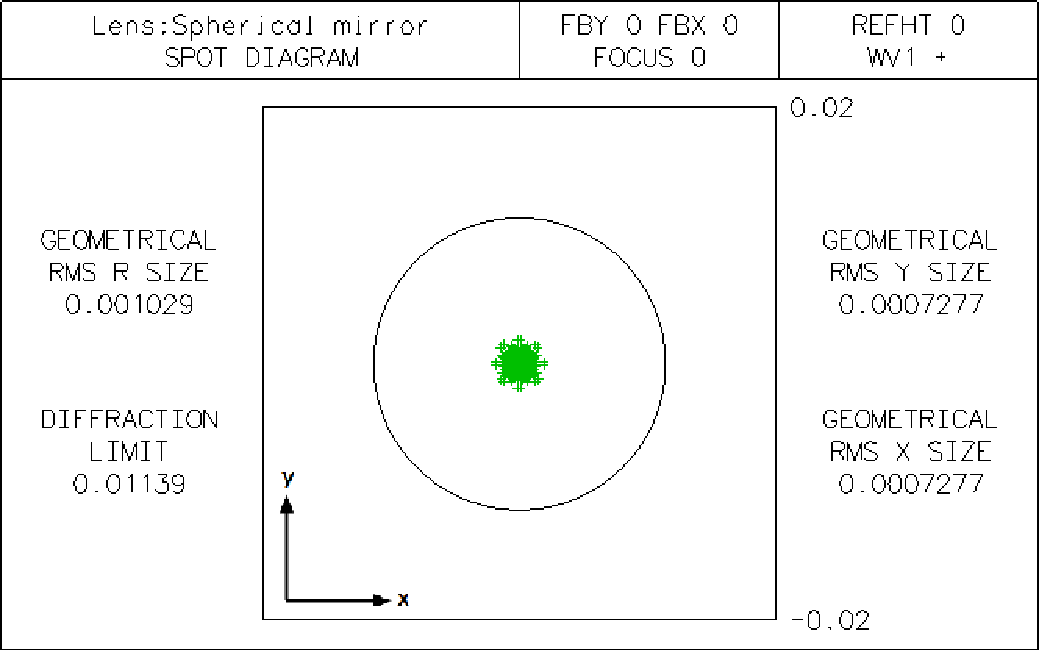
\includegraphics[scale=0.5]{figure/off_axis_spot_0.pdf}
    \caption{凹面鏡で集光した際の焦点面でのスポット図(同軸で集光)}
    \label{fig:off_axis_spot_0}
\end{figure}
\begin{figure}[htbp]
    \centering
    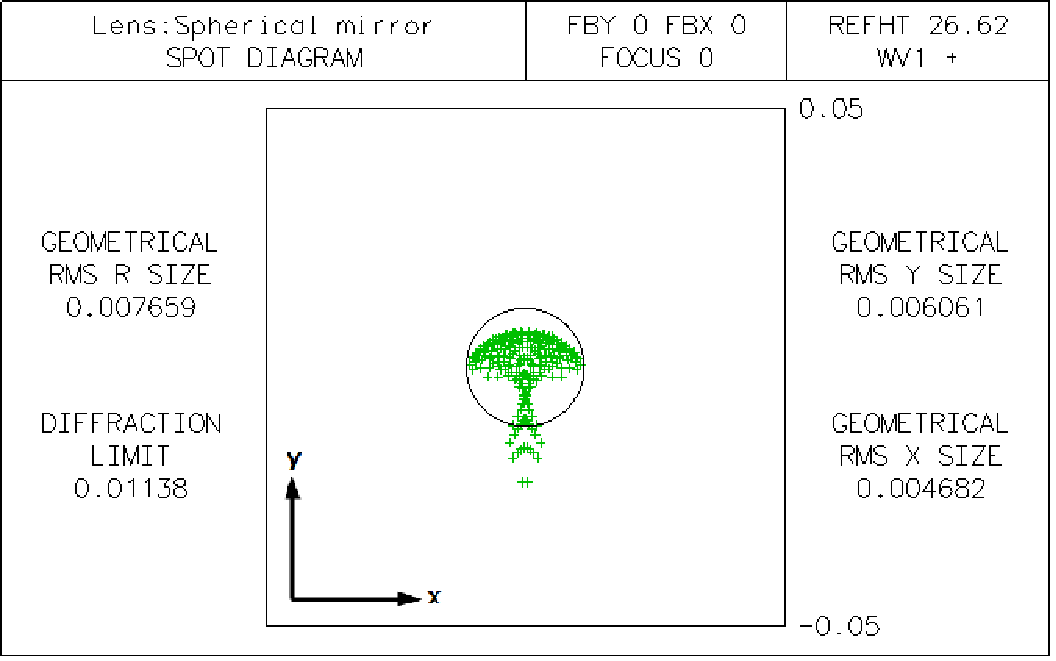
\includegraphics[scale=0.5]{figure/off_axis_spot_1.pdf}
    \caption{凹面鏡で集光した際の焦点面でのスポット図(軸外反射の角度を2°に設定)}
    \label{fig:off_axis_spot_1}
\end{figure}
\begin{figure}[htbp]
    \centering
    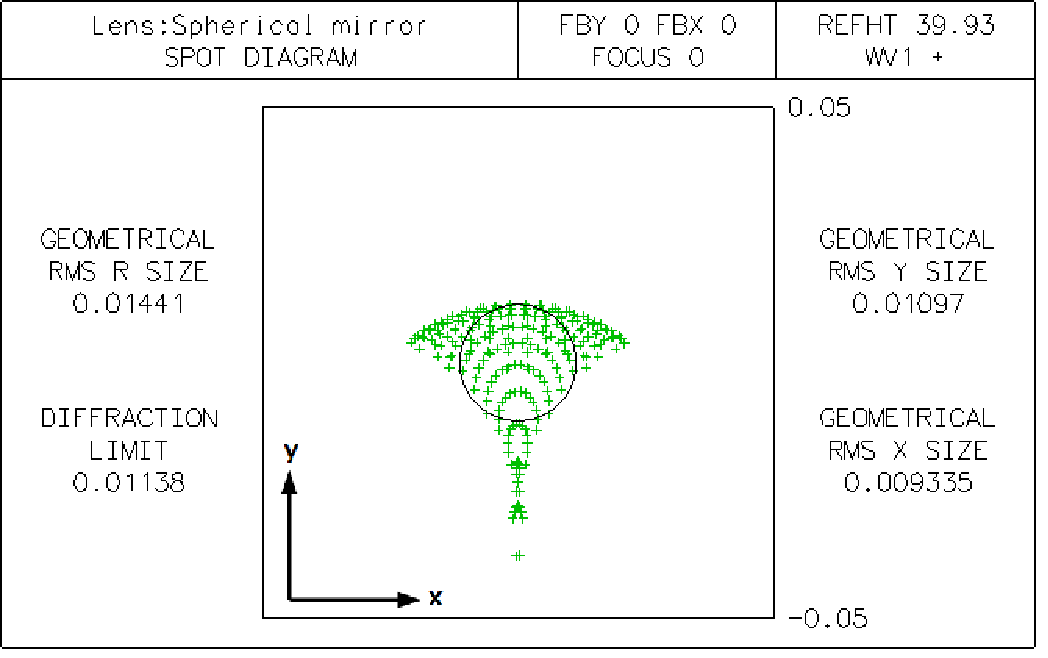
\includegraphics[scale=0.5]{figure/off_axis_spot_1.5.pdf}
    \caption{凹面鏡で集光した際の焦点面でのスポット図(軸外反射の角度を3°に設定)}
    \label{fig:off_axis_spot_1.5}
\end{figure}
\begin{figure}[htbp]
    \centering
    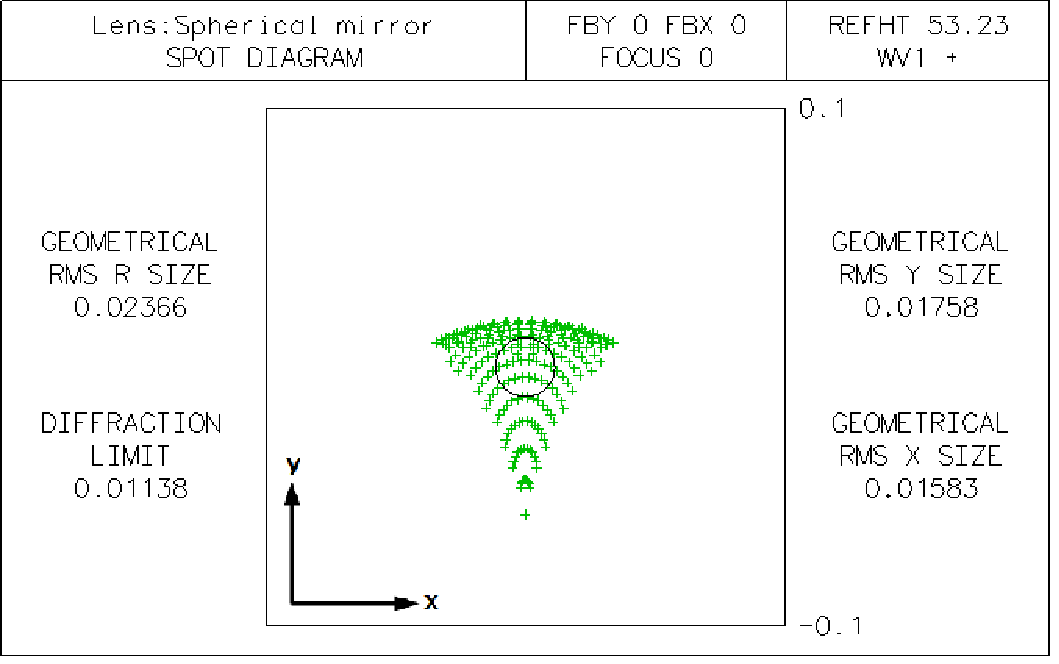
\includegraphics[scale=0.5]{figure/off_axis_spot_2.pdf}
    \caption{凹面鏡で集光した際の焦点面でのスポット図(軸外反射の角度を4°に設定)}
    \label{fig:off_axis_spot_2}
\end{figure}
図中の円はエアリーディスクを表す.
これらの図を見ると軸外反射の角度を大きくするほど結像が大きくなることがよくわかる.
% 同軸で集光した際の結像である図\ \ref{fig:off_axis_spot_0}を見ると全ての光線がエアリーディスク内に集まっているため回折限界で集光できると言える.
% 対して図\ \ref{fig:off_axis_spot_2}のように軸外反射の角度を4°に設定し集光した場合,光はエアリーディスクから大きくはみ出しており,収差の影響を受けることが分かる.

ツェルニ・ターナ型分光器では2つの凹面鏡を近付けるほど軸外反射の角度を小さくすることができる.
また同様に凹面鏡から回折格子までの距離を離せば離すほど軸外反射の角度を小さくすることができるが,一般に回折格子が回転するための余裕などを考え凹面鏡と回折格子の距離を凹面鏡の焦点距離の7~8割程度にして配置しているものが多い.
今回設定した焦点距離を1525 mm,有効径を98 mmの凹面鏡を用いて凹面鏡から回折格子までの距離を焦点距離の8割である1220 mmにすると,二つの凹面鏡を可能な限り近づけて配置しても軸外反射の角度は計算上約2.8°となる.
実際には二つの凹面鏡は少し離れて設置しないと回折格子が光路を遮ってしまうので軸外反射の角度は最小で3°ほどになると考えられる.

図\ \ref{fig:off_axis_spot_1.5}のように軸外反射の角度を3°に設定し集光した場合,光はエアリーディスクからはみ出しており,収差の影響を受けることが分かる.
従って,ツェルニターナ型の分光器の配置では焦点距離が1525 mmと長い凹面鏡を使用しても回折限界での集光は難しく,分解能が収差の影響を受ける.


\subsection{アクロマティックレンズを用いた結像}

次章で述べるように本研究ではコリメータ及び結像器にアクロマティックレンズを使用する.
アクロマティックレンズとは異なる二つのレンズが組み合わされたレンズである.
一般に低屈折率ガラスを用いた正レンズと高屈折率のガラスを用いた負レンズで構成されている.

% アクロマティックレンズの特徴として色収差が補正されているという点がある.
アクロマティックレンズでは構成する2つのレンズが補完しあうことにより,単レンズと比べて色収差を抑えることができる.
図\ \ref{fig:achromaticlense}にアクロマティックレンズが色収差を抑えている様子の簡易図を示す.
\begin{figure}[htbp]
    \centering
    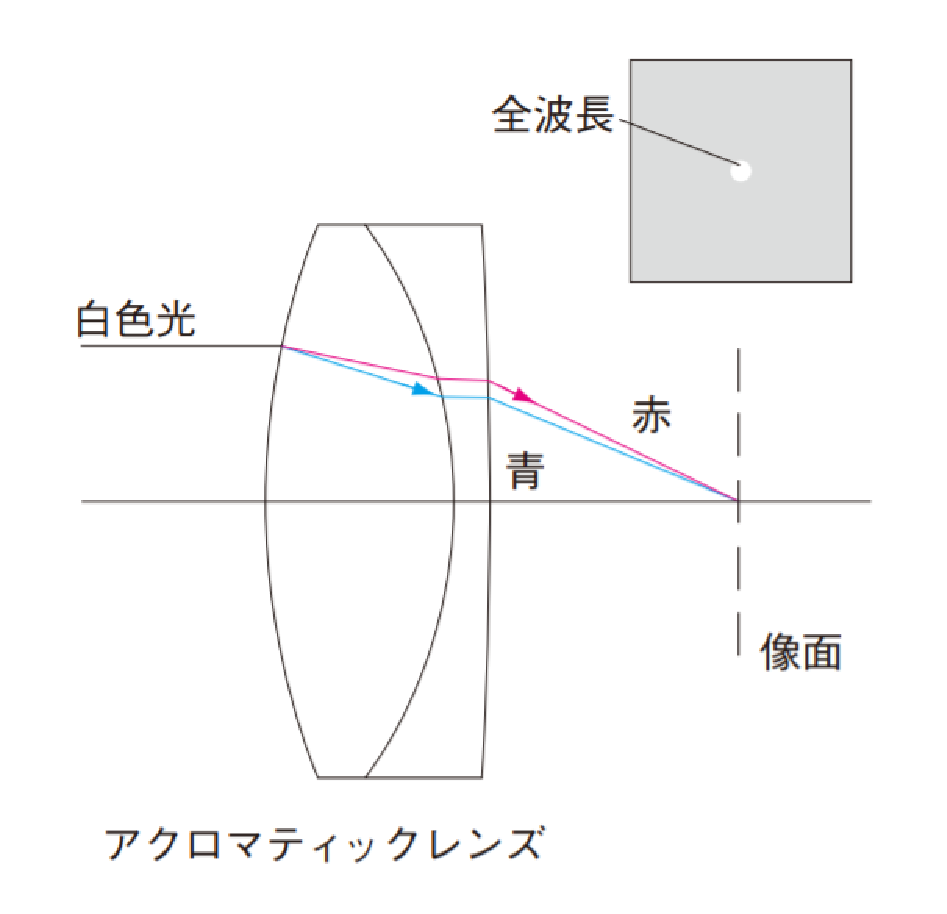
\includegraphics[scale=0.6]{figure/achromaticlense.pdf}
    \caption{アクロマティックレンズでの集光の模式図\cite{achromatic_lens}}
    \label{fig:achromaticlense}
\end{figure}
また,同様に色収差のみでなく球面収差も改善されており,レンズの有効径が大きい場合でも単レンズと比べて小さな結像を得ることができる\cite{achromatic_lens}.


本研究で使用するレンズに平行光を入射させた際の焦点面でのスポット図を図\ \ref{fig:lens_spot}に示す.
\begin{figure}[htbp]
    \centering
    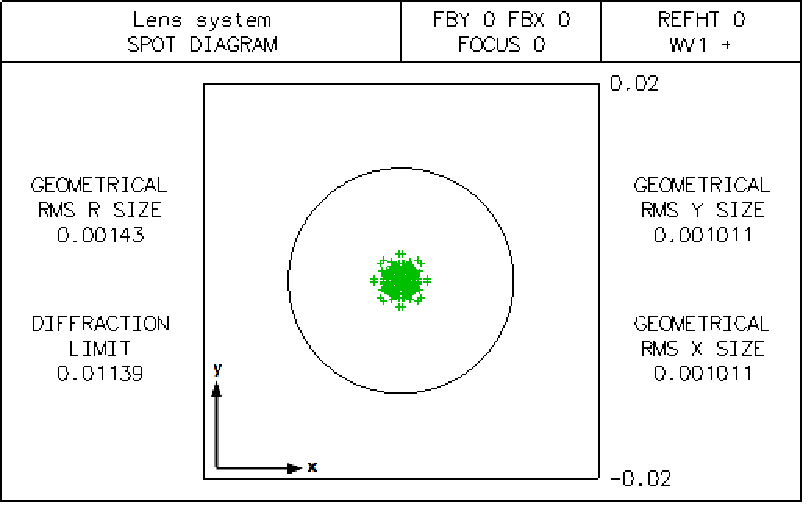
\includegraphics[scale=0.6]{figure/lens_spot.pdf}
    \caption{本分光器の使用レンズで光を同軸に集光した際の焦点面でのスポット図}
    \label{fig:lens_spot}
\end{figure}
全ての光線がエアリーディスク内に集まっているため,回折限界で集光されていると言える.

% 本研究での使用レンズは高い集光性能を持っており,結像面の中心に近いほど光線が多く集まる.
% よって,結像の中心ほど明るくなっている.
結像面における光の分布(光の強度)が二次元のガウス関数で近似できるとすると,スポット図にあるGEOMETRICAL RMS R SIZE($rms_r$と置く)は半径方向の二乗平均平方根であり,ガウス関数の標準偏差$\sigma$に対応する.
この際,結像の大きさ$\phi$を光の分布図をガウス関数に近似した際の半値全幅と定義すると
\begin{eqnarray}
     \phi &=& 2rms_r \sqrt{2\log2} \nonumber \\
     &\simeq&2.35rms_r
\end{eqnarray}
とできる.
以下では,本研究で使用しているレンズの作る設計上の像の大きさをこの$\phi$で定義する.